% Written by projects/review-walk/paper/generate.mjs; do not edit by hand.

\newcommand{\AppCommit}{e06307fe45}
\newcommand{\MaxErrors}{four}
\newcommand{\QuietErrors}{two}
\newcommand{\MaxHonors}{one}
\newcommand{\MateWithin}{three}
\newcommand{\LongWalk}{five}
\newcommand{\MaxStops}{five}
\newcommand{\HeldBefore}{2026-09-23}
\newcommand{\HeldAsked}{80}
\newcommand{\Draws}{10,000}
\newcommand{\MedianAbove}{50}
\newcommand{\QuartileBar}{40}
\newcommand{\TurnBar}{90}
\newcommand{\DesignGames}{734}
\newcommand{\DesignWithErrors}{707}
\newcommand{\DesignMomentsMedian}{6}
\newcommand{\DesignMomentsNinety}{11.7}
\newcommand{\DesignMomentsMost}{30}
\newcommand{\DesignStopsMedian}{3}
\newcommand{\DesignStopsNinety}{4}
\newcommand{\DesignStopsMost}{5}
\newcommand{\DesignLonger}{54}
\newcommand{\DesignNoStops}{19}
\newcommand{\DesignCoverage}{72}
\newcommand{\DesignCoverageLow}{70}
\newcommand{\DesignCoverageHigh}{73}
\newcommand{\DesignQuartile}{59}
\newcommand{\DesignTenth}{48}
\newcommand{\DesignSeriousGames}{636}
\newcommand{\DesignSeriousWhole}{71}
\newcommand{\DesignSeriousTenth}{77}
\newcommand{\DesignSeenIn}{707}
\newcommand{\DesignSeenOf}{707}
\newcommand{\DesignSeenAt}{63}
\newcommand{\DesignSeenAtLow}{28}
\newcommand{\DesignSeenAtHigh}{95}
\newcommand{\DesignTurnIn}{340}
\newcommand{\DesignTurnOf}{346}
\newcommand{\DesignTurnShare}{98}
\newcommand{\DesignMates}{27}
\newcommand{\DesignHonors}{173}
\newcommand{\DesignFirstStop}{39}
\newcommand{\DesignByCost}{87}
\newcommand{\DesignSoftened}{3}
\newcommand{\DesignFourthAdds}{4.6}
\newcommand{\DesignFifthAdds}{3.5}
\newcommand{\HeldGames}{80}
\newcommand{\HeldWithErrors}{79}
\newcommand{\HeldMomentsMedian}{6}
\newcommand{\HeldMomentsNinety}{11}
\newcommand{\HeldMomentsMost}{14}
\newcommand{\HeldStopsMedian}{3}
\newcommand{\HeldStopsNinety}{4}
\newcommand{\HeldStopsMost}{5}
\newcommand{\HeldLonger}{54}
\newcommand{\HeldNoStops}{1}
\newcommand{\HeldCoverage}{76}
\newcommand{\HeldCoverageLow}{70}
\newcommand{\HeldCoverageHigh}{79}
\newcommand{\HeldQuartile}{64}
\newcommand{\HeldTenth}{55}
\newcommand{\HeldSeriousGames}{70}
\newcommand{\HeldSeriousWhole}{71}
\newcommand{\HeldSeriousTenth}{83}
\newcommand{\HeldSeenIn}{79}
\newcommand{\HeldSeenOf}{79}
\newcommand{\HeldSeenAt}{59}
\newcommand{\HeldSeenAtLow}{30}
\newcommand{\HeldSeenAtHigh}{93}
\newcommand{\HeldTurnIn}{37}
\newcommand{\HeldTurnOf}{37}
\newcommand{\HeldTurnShare}{100}
\newcommand{\HeldMates}{4}
\newcommand{\HeldHonors}{14}
\newcommand{\HeldFirstStop}{38}
\newcommand{\HeldByCost}{88}
\newcommand{\HeldSoftened}{1}
\newcommand{\HeldFourthAdds}{6.7}
\newcommand{\HeldFifthAdds}{3.9}
\newcommand{\TeachStops}{212}
\newcommand{\TeachCards}{212}
\newcommand{\TeachCardShare}{100}
\newcommand{\TeachReply}{115}
\newcommand{\TeachReplyShare}{54}
\newcommand{\TeachChance}{50}
\newcommand{\TeachChanceShare}{24}
\newcommand{\TeachNeither}{47}
\newcommand{\TeachNeitherShare}{22}
\newcommand{\TeachLesson}{199}
\newcommand{\TeachLessonShare}{94}
\newcommand{\Kept}{kept}
\newcommand{\CheckMedian}{holds}
\newcommand{\CheckQuartile}{holds}
\newcommand{\CheckTurn}{holds}
\newcommand{\CheckLength}{holds}
\newcommand{\CheckSeen}{holds}
\newcommand{\MeasureTable}{%
\begin{table}[h]\centering\small
\begin{tabular}{lrr}
\toprule
 & design set & held out \\
\midrule
games & 734 & 80 \\
his marked moves a game: median, 90th, most & 6, 11.7, 30 & 6, 11, 14 \\
the walk's stops: median, 90th, most & 3, 4, 5 & 3, 4, 5 \\
games with more than five marked moves & 54\% & 54\% \\
cost held, median game (95\% interval) & 72\% (70 to 73) & 76\% (70 to 79) \\
cost held, lower-quartile game & 59\% & 64\% \\
a stop inside the turn, of games that turned on his moves & 340 of 346 & 37 of 37 \\
the costliest error is a stop & 707 of 707 & 79 of 79 \\
mistakes, misses and blunders all held & 71\% of 636 & 71\% of 70 \\
\bottomrule
\end{tabular}
\caption{The walk on the design set (the archive's reviews) and on the held-out phone reviews. Cost held is the \texttt{lossPct} of the errors the walk stops at over that of all his errors, inaccuracies included.}
\label{tab:measures}
\end{table}
}
\newcommand{\CapFigure}{%
\begin{figure}[h]\centering
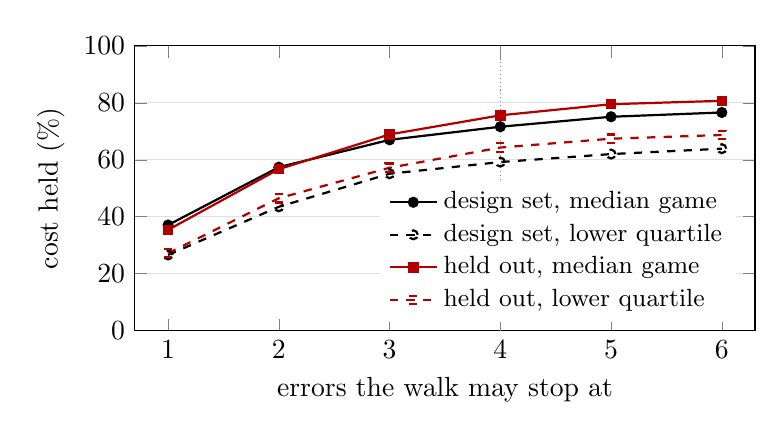
\begin{tikzpicture}
\begin{axis}[width=0.78\linewidth, height=5.2cm, xmin=0.7, xmax=6.3, ymin=0, ymax=100, xtick={1,2,3,4,5,6}, xlabel={errors the walk may stop at}, ylabel={cost held (\%)}, legend pos=south east, legend cell align=left, legend style={font=\small, draw=none}, ymajorgrids, grid style={black!12}]
\addplot[thick, black, mark=*, mark size=1.6pt] coordinates {(1,37.1) (2,57.4) (3,67.0) (4,71.6) (5,75.1) (6,76.6)};
\addlegendentry{design set, median game}
\addplot[thick, black, dashed, mark=o, mark size=1.6pt] coordinates {(1,26.6) (2,43.5) (3,55.1) (4,59.2) (5,62.0) (6,63.9)};
\addlegendentry{design set, lower quartile}
\addplot[thick, red!70!black, mark=square*, mark size=1.5pt] coordinates {(1,35.4) (2,56.7) (3,68.9) (4,75.6) (5,79.5) (6,80.7)};
\addlegendentry{held out, median game}
\addplot[thick, red!70!black, dashed, mark=square, mark size=1.5pt] coordinates {(1,27.2) (2,46.5) (3,57.2) (4,64.3) (5,67.4) (6,68.7)};
\addlegendentry{held out, lower quartile}
\draw[black!45, densely dotted] (axis cs:4,0) -- (axis cs:4,100);
\end{axis}
\end{tikzpicture}
\caption{What the walk would hold of what his errors cost if it stopped at one to six of them, ranked as the walk ranks them. The dotted line is the cap the app uses.}
\label{fig:caps}
\end{figure}
}
